\subsection{Makerere University}

Como siguiente caso de estudio se eligió la Universidad Makerere de Uganda, alojada en \emph{mak.ac.ug}. Las mediciones fueron realizadas en varias oportunidades utilizando 30 iteraciones por TTL para garantizar la confiabilidad de los datos.

En la figura \ref{fig:makerere-incrementales} se aprecian las mediciones de las RTTs.

\begin{figure}[H]
    \centering
    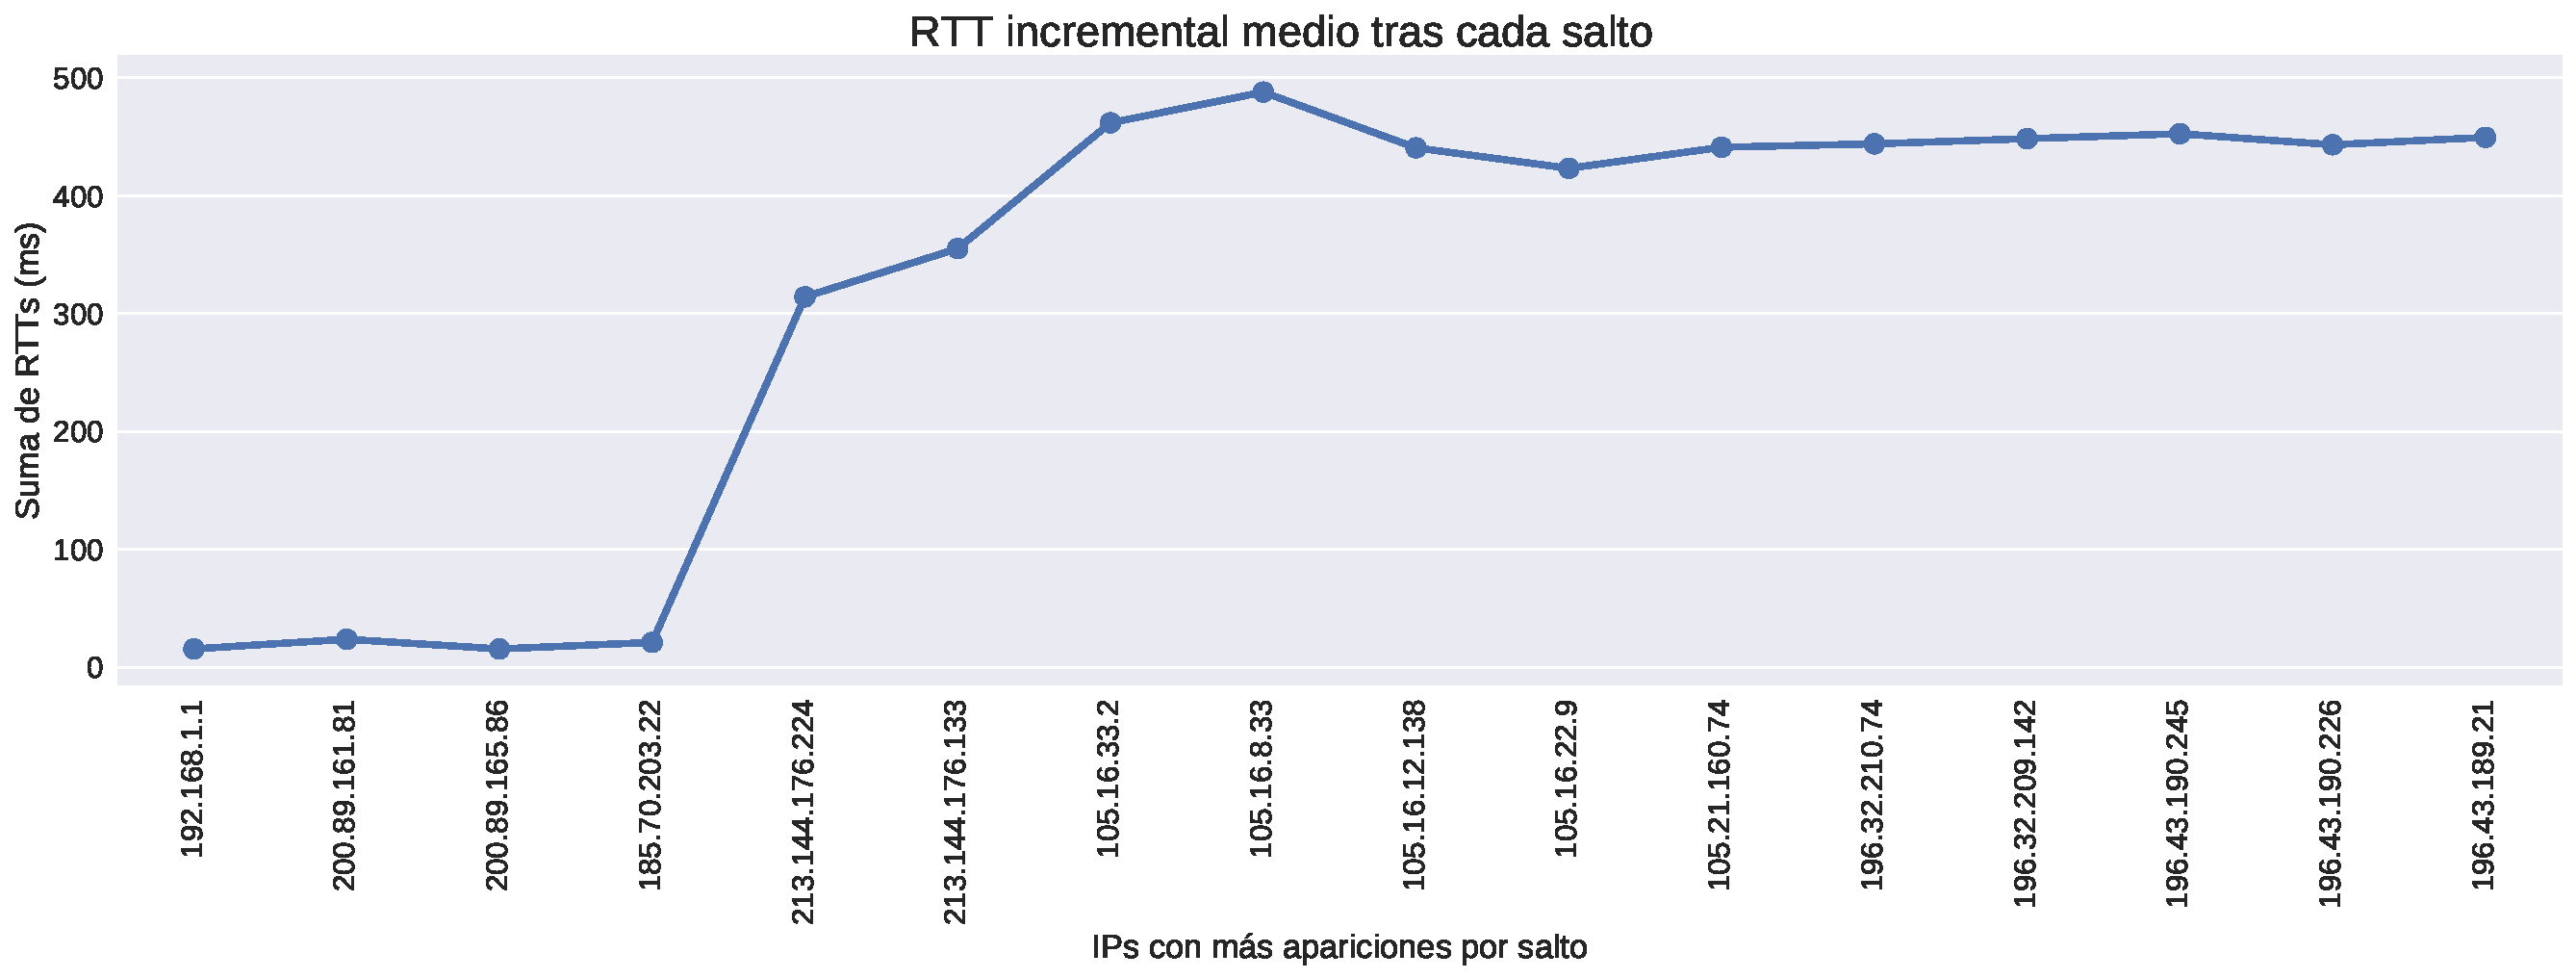
\includegraphics[width=1\textwidth, height=1\textheight, keepaspectratio]{../img/mak-ac-ug-incrementales}
    \caption{Comportamiento incremental de RTTs medios medidos.}
    \label{fig:makerere-incrementales}
\end{figure}

Nos encontramos primero con un segmento con delay que pareciera corresponder a servidores locales, aunque vemos que la última ip ($185.70.203.22$) se geolocaliza en Italia. La siguiente ip ($213.144.176.244$) corresponde también a coordenadas italianas, por lo que suponemos que se trata de los dos extremos de un cable submarino.

El siguiente salto se produce en la ip $105.16.33.2$, que parece ahora ubicarse en Francia.
Las siguientes dos ips nos llevan a la isla de Mauricio, pero no se corresponde con una diferencia notable en RTTs. Esto sumado a la similitud de estas ips con la francesa nos mueve a pensar que se trata de un cable submarino desde Italia a Mauricio, y que la ip francesa aparece por alguna razón interna de la empresa correspondiente.

Luego tenemos una sucesión de ips de Tanzania, Sudáfrica y finalmente Uganda, con poca diferencia de RTTs por lo que suponemos que se trata del enlace terrestre final.

En la figura \ref{fig:makerere-rtts} vemos mas directamente estas diferencias de RTT.

\begin{figure}[H]
   \centering
       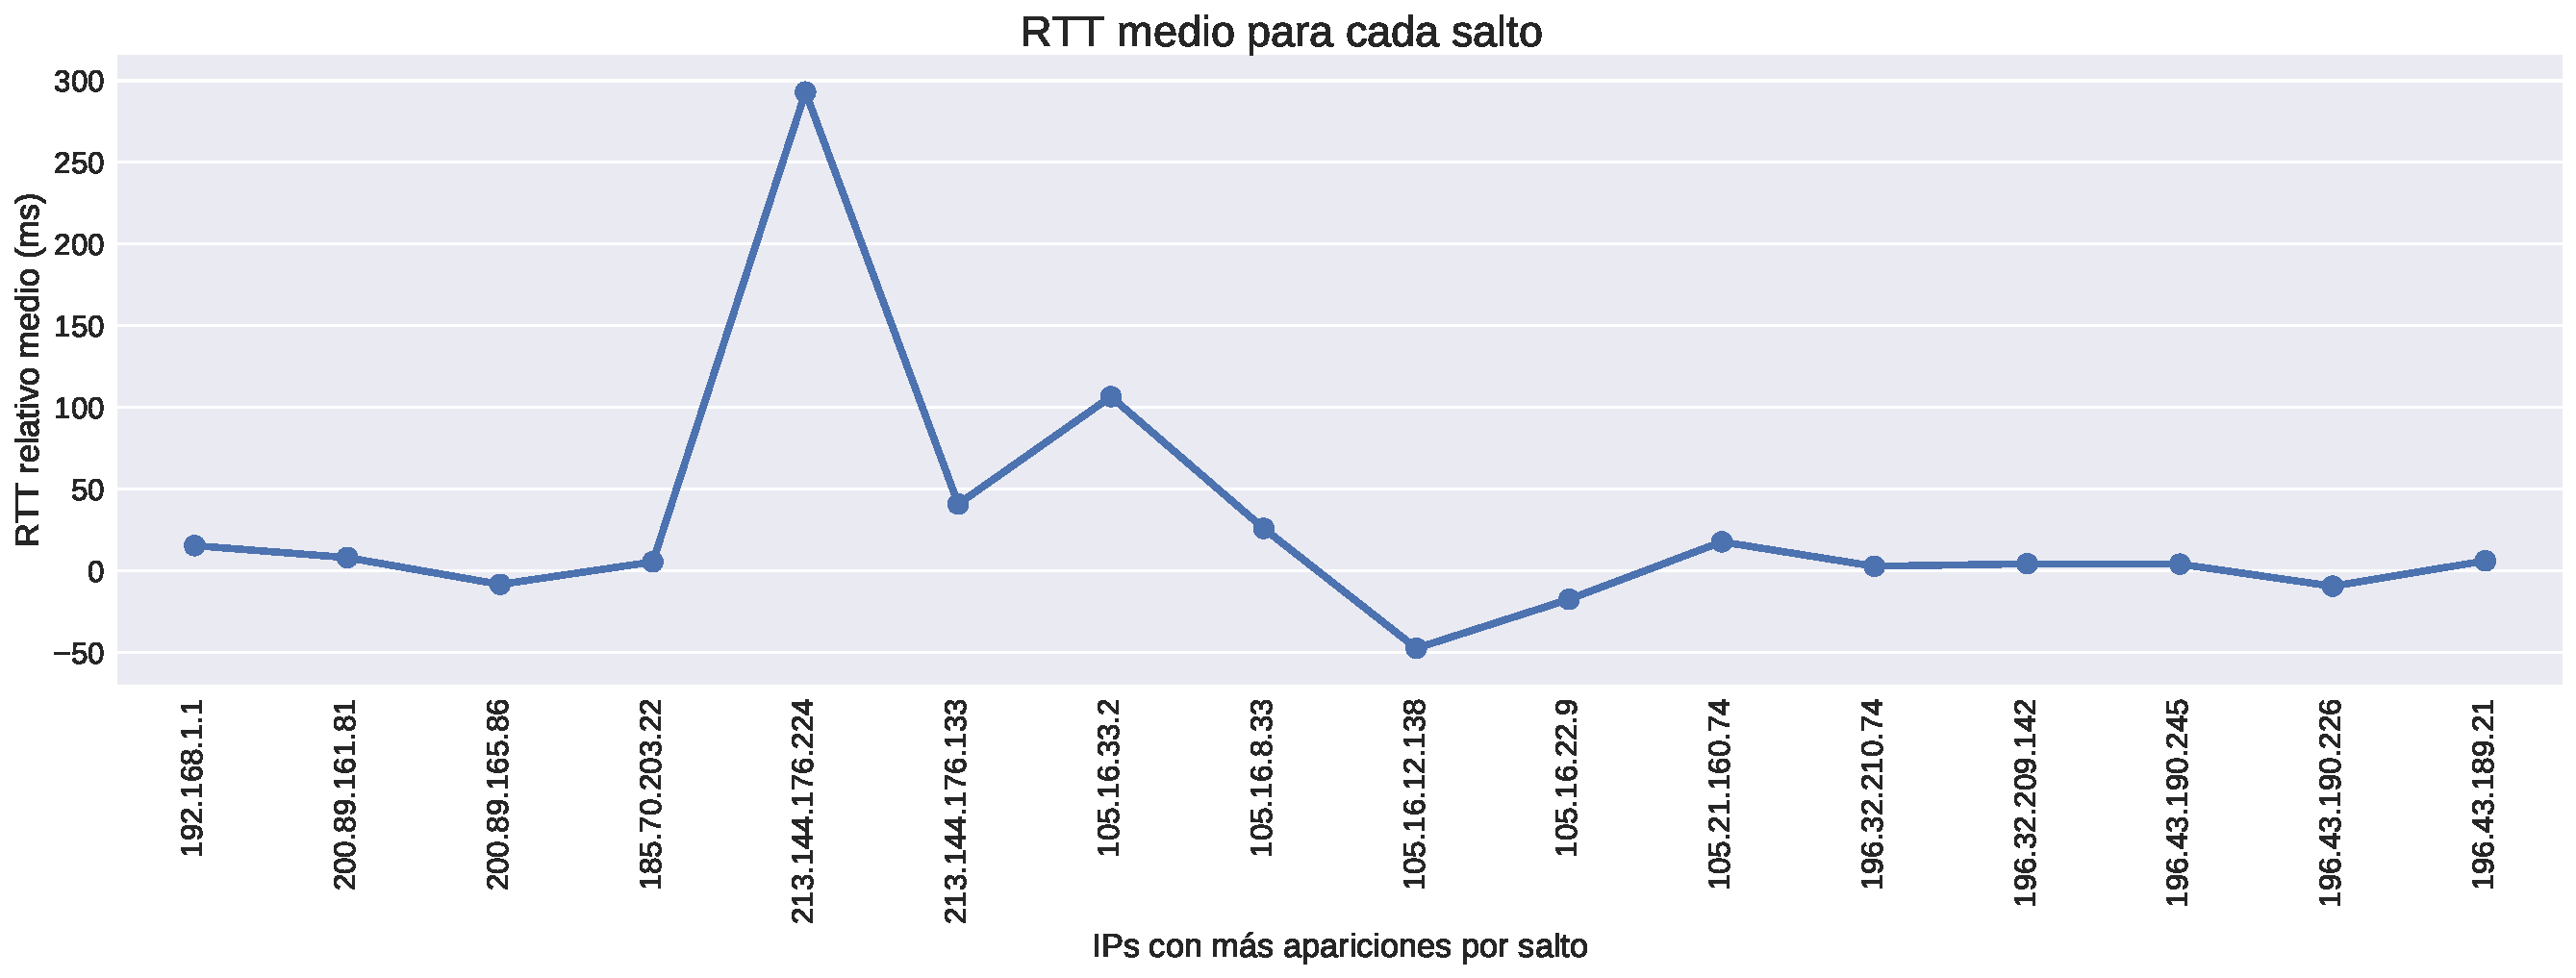
\includegraphics[width=1\textwidth, height=1\textheight, keepaspectratio]{../img/mak-ac-ug-rtts}
 \caption{RTTs medios medidos para una traceroute a la Universidad Makerere}
 \label{fig:makerere-rtts}
\end{figure}

Graficamos esta ruta en el mapa de la figura \ref{makerere-map}, donde los caminos mas rojos se corresponden con una diferencia de RTT mayor.

\begin{figure}[H]
   \centering
       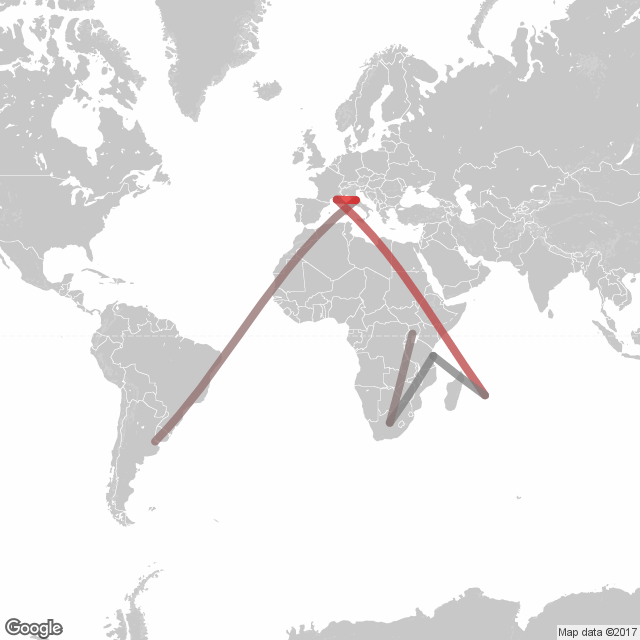
\includegraphics[width=0.6\textwidth, keepaspectratio]{../img/mak-ac-ug-map}
 \caption{Mapa de ubicaciones inferidas para una traceroute a la Universidad Makerere}
 \label{fig:makerere-map}
\end{figure}

En total 16 de los 20 nodos del camino (\textbf{80}\%) respondieron a la herramienta del traceroute.

Para terminar utilizamos el método de Cimbala para detectar cables submarinos en la ruta. El resultado, que puede verse en la figura \ref{fig:makerere-zrtt} nos marca claramente el cable desde Argentina a Italia. Ademas, viendo el umbral $1$ detectamos el cable que suponemos desde Italia a Mauricio y un segundo cable que debe corresponderse con el tramo Mauricio-Tanzania.
 
\begin{figure}[H]
   \centering
       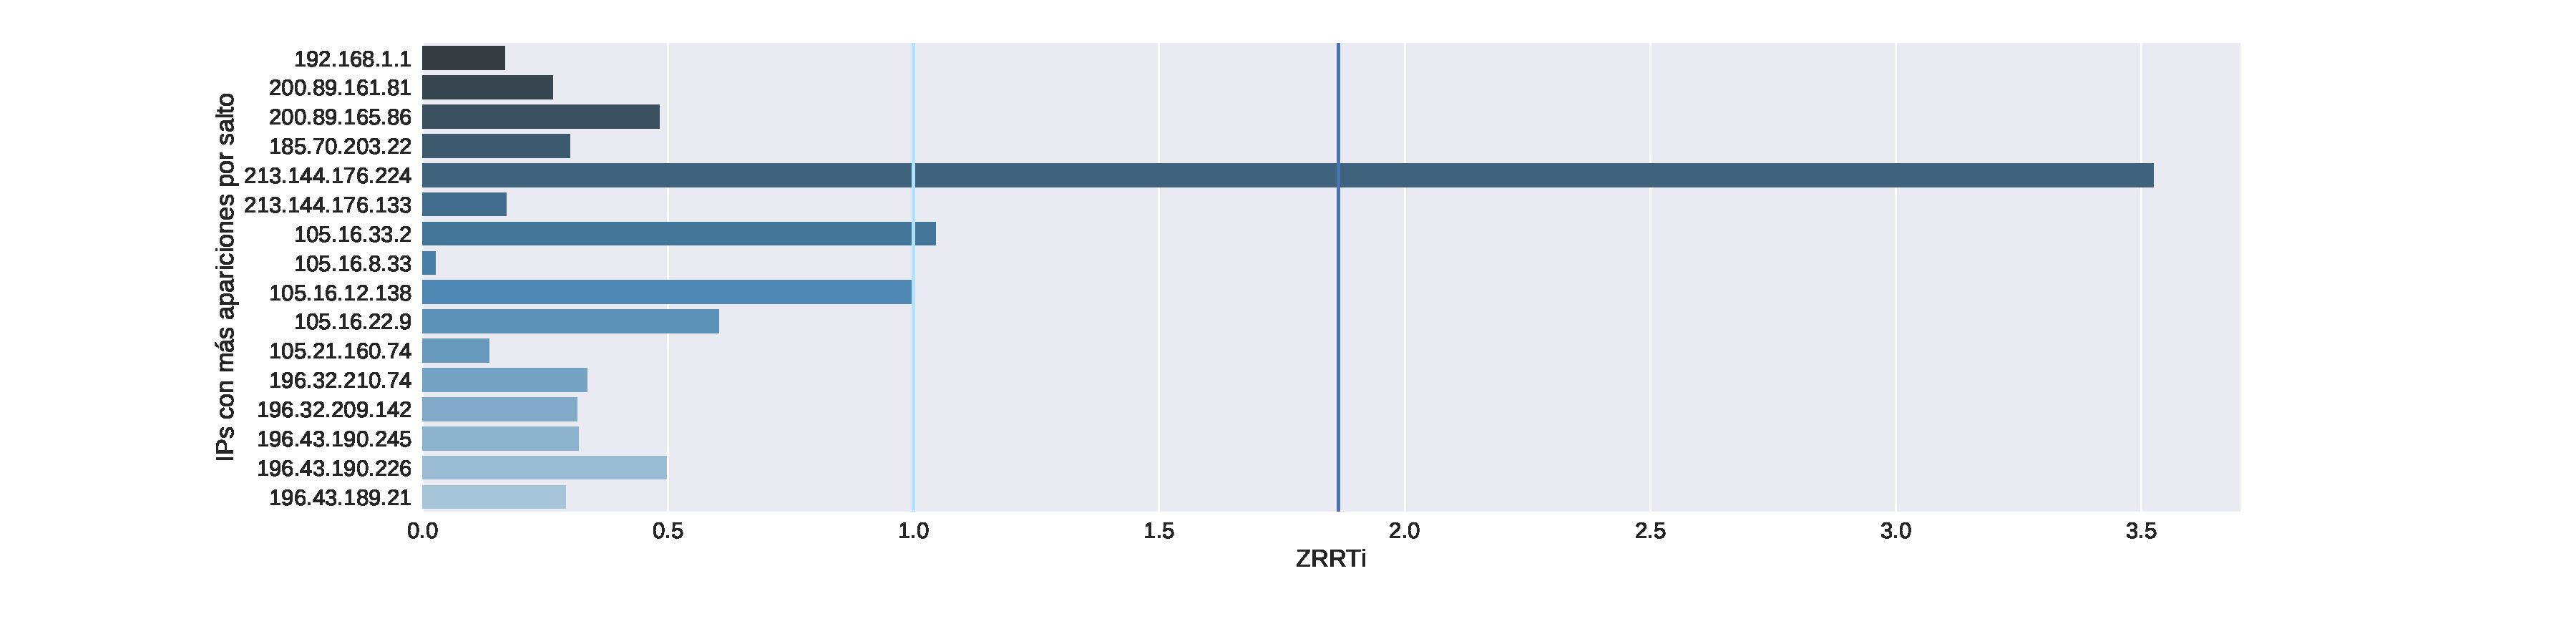
\includegraphics[width=1\textwidth, height=1\textheight, keepaspectratio]{../img/mak-ac-ug-zrtt}
 \caption{Outliers de la distribución ZRRTi según el método de Cimbala. En azul oscuro: valor $ZRTT_i$ correspondiente a $\tau(n)$ con $n$ el largo de ruta y un alfa fijo (0.05 sugerido en el paper de referencia).}
 \label{fig:makerere-zrtt}
\end{figure}

